\section{Sequences} \label{S:7.1.Sequences}

\begin{goals}
\item What is a sequence?
\item What does it mean for a sequence to converge?
\item What does it mean for a sequence to diverge?
\end{goals}

%-----------------------------------
% SUBSECTION INTRODUCTION
%-----------------------------------
\subsection*{Introduction}

We encounter sequences every day. Your monthly rent payments, the annual interest you earn on investments, a list of your car's miles per gallon every time you fill up; all are examples of sequences. Other sequences with which you may be familiar include the Fibonacci sequence\index{Fibonacci sequence}
\[1, 1, 2, 3, 5, 8, \ldots\]
in which each entry is the sum of the two preceding entries and the triangular numbers\index{triangular numbers}
\[1, 3, 6, 10, 15, 21, 28, 36, 45, 55, \ldots\]
which are numbers that correspond to the number of vertices seen in the triangles in Figure \ref{F:8.1.Triangular_numbers}.
\begin{marginfigure} % MARGIN FIGURE
\margingraphics{figures/8_1_Triangular_Numbers.eps}
\caption{Triangular numbers}
\label{F:8.1.Triangular_numbers}
\end{marginfigure}
Sequences of integers are of such interest to mathematicians and others that they have a journal\footnote{\emph{The Journal of Integer Sequences} at \url{http://www.cs.uwaterloo.ca/journals/JIS/}} devoted to them and an on-line encyclopedia\footnote{The On-Line Encyclopedia of Integer Sequences at \url{http://oeis.org/}} that catalogs a huge number of integer sequences and their connections. Sequences are also used in digital recordings and digital images. 

To this point, most of our studies in calculus have dealt with continuous information (e.g., continuous functions). The major difference we will see now is that sequences model \emph{discrete} instead of continuous information. We will study ways to represent and work with discrete information in this chapter as we investigate \emph{sequences} and \emph{series}, and ultimately see key connections between the discrete and continuous.

\begin{margintable}[8cm]
\begin{center}
%\renewcommand{\arraystretch}{1.5}
\begin{tabular}{|c|c|c|} \hline
Month   &Interest earned    &Total amount \\ \hline
$0$       &$\$0$              &$\$5000.00$  \\ \hline
$1$       &$\$33.33$          &$\$5033.33$  \\ \hline
$2$       &                   &\\ \hline
$3$       &                   &\\ \hline
$4$       &                   &\\ \hline
$5$       &                   &\\ \hline
$6$       &                   &\\ \hline
$7$       &                   &\\ \hline
$8$       &                   &\\ \hline
$9$       &                   &\\ \hline
$10$      &                   &\\ \hline
$11$      &                   &\\ \hline
$12$      &                   &\\ \hline
\end{tabular}
\caption{Interest}
\label{T:PA_8.1.Interest}
\end{center}
\end{margintable}

\begin{pa} \label{PA:8.1}
Suppose you receive $\$5000$ through an inheritance. You decide to invest this money into a fund that pays $8\%$ annually, compounded monthly. That means that each month your investment earns $\frac{0.08}{12} \cdot P$ additional dollars, where $P$ is your principal balance at the start of the month. So in the first month your investment earns
\[5000 \left(\frac{0.08}{12}\right)\]
or $\$33.33$. If you reinvest this money, you will then have $\$5033.33$ in your account at the end of the first month. From this point on, assume that you reinvest all of the interest you earn.
    \ba
    \item How much interest will you earn in the second month? How much money will you have in your account at the end of the second month?

    \item Complete Table \ref{T:PA_8.1.Interest} to determine the interest earned and total amount of money in this investment each month for one year.

    \item As we will see later, the amount of money $P_n$ in the account after month $n$ is given by
    \[P_n = 5000\left(1+\frac{0.08}{12}\right)^{n}.\]
    Use this formula to check your calculations in Table \ref{T:PA_8.1.Interest}. Then find the amount of money in the account after $5$ years.
    
    \item How many years will it be before the account has doubled in value to $\$10000$?

\ea
\end{pa}
\afterpa  % PREVIEW ACTIVITY

%-------------------------------
% SUBSECTION SEQUENCES
%-------------------------------
\subsection*{Sequences} \index{sequence}

As our discussion in the introduction and Preview Activity \ref{PA:8.1} illustrate, many discrete phenomena can be represented as lists of numbers (like the amount of money in an account over a period of months). We call these any such list a \emph{sequence}. In other words, a sequence is nothing more than list of terms in some order. To be able to refer to a sequence in a general sense, we often list the entries of the sequence with subscripts,
\[s_1, s_2, \ldots, s_n \ldots,\]
where the subscript denotes the position of the entry in the sequence. More formally,

\definition{Sequence}{ % DEFINITION
A sequence is a list of terms $s_1, s_2, s_3, \ldots$ in a specified order. 
} % end definition

As an alternative to the above definition, we can also consider a sequence to be a function $f$ whose domain is the set of positive integers. In this context, the sequence $s_1$, $s_2$, $s_3$, $\ldots$ would correspond to the function $f$ satisfying $f(n) = s_n$ for each positive integer $n$. This alternative view will be be useful in many situations. 

We will often write the sequence
\[s_1, s_2, s_3, \ldots\]
using the shorthand notation $\{s_n\}$. The value $s_n$ (alternatively $s(n)$) is called the $n$th \emph{term}\index{sequence!term} in the sequence. If the terms are all 0 after some fixed value of $n$, we say the sequence is finite. Otherwise the sequence is infinite. We will work with both finite and infinite sequences, but focus more on the infinite sequences. With infinite sequences, we are often interested in their end behavior and the idea of \emph{convergent} sequences.

\begin{activity} \label{7.1.Act1}
\ba
\item Let $s_n$ be the $n$th term in the sequence $1, 2, 3, \ldots$. 

Find a formula for $s_n$ and use appropriate technological tools to draw a graph of entries in this sequence by plotting points of the form $(n,s_n)$ for some values of $n$. Most graphing calculators can plot sequences; directions follow for the TI-84.
\begin{itemize}
\item In the MODE menu, highlight SEQ in the FUNC line and press ENTER.
\item In the Y= menu, you will now see lines to enter sequences. Enter a value for $n$Min (where the sequence starts), a function for $u(n)$ (the $n$th term in the sequence), and the value of $u_{n\text{Min}}$.
\item Set your window coordinates (this involves choosing limits for $n$ as well as the window coordinates XMin, XMax, YMin, and YMax.
\item The GRAPH key will draw a plot of your  sequence.
\end{itemize}
Using your knowledge of limits of continuous functions as $x \to \infty$, decide if this sequence $\{s_n\}$ has a limit as $n \to \infty$. Explain your reasoning.

\item Let $s_n$ be the $n$th term in the sequence $1, \frac{1}{2}, \frac{1}{3}, \ldots$. Find a formula for $s_n$. Draw a graph of some points in this sequence. Using your knowledge of limits of continuous functions as $x \to \infty$, decide if this sequence $\{s_n\}$ has a limit as $n \to \infty$. Explain your reasoning.

\item Let $s_n$ be the $n$th term in the sequence $2, \frac{3}{2}, \frac{4}{3}, \frac{5}{4}, \ldots$. Find a formula for $s_n$. Using your knowledge of limits of continuous functions as $x \to \infty$, decide if this sequence $\{s_n\}$ has a limit as $n \to \infty$. Explain your reasoning.

\ea
\end{activity}

\begin{smallhint}
\ba
	\item Small hints for each of the prompts above.
\ea
\end{smallhint}
\begin{bighint}
\ba
	\item Big hints for each of the prompts above.
\ea
\end{bighint}
\begin{activitySolution}
\ba
	\item By observation we see that a formula for $s_n$ is $s_n = n$. A plot of the first 50 points in the sequence is shown here.
%\begin{center} 
%\resizebox{!}{1.75in}{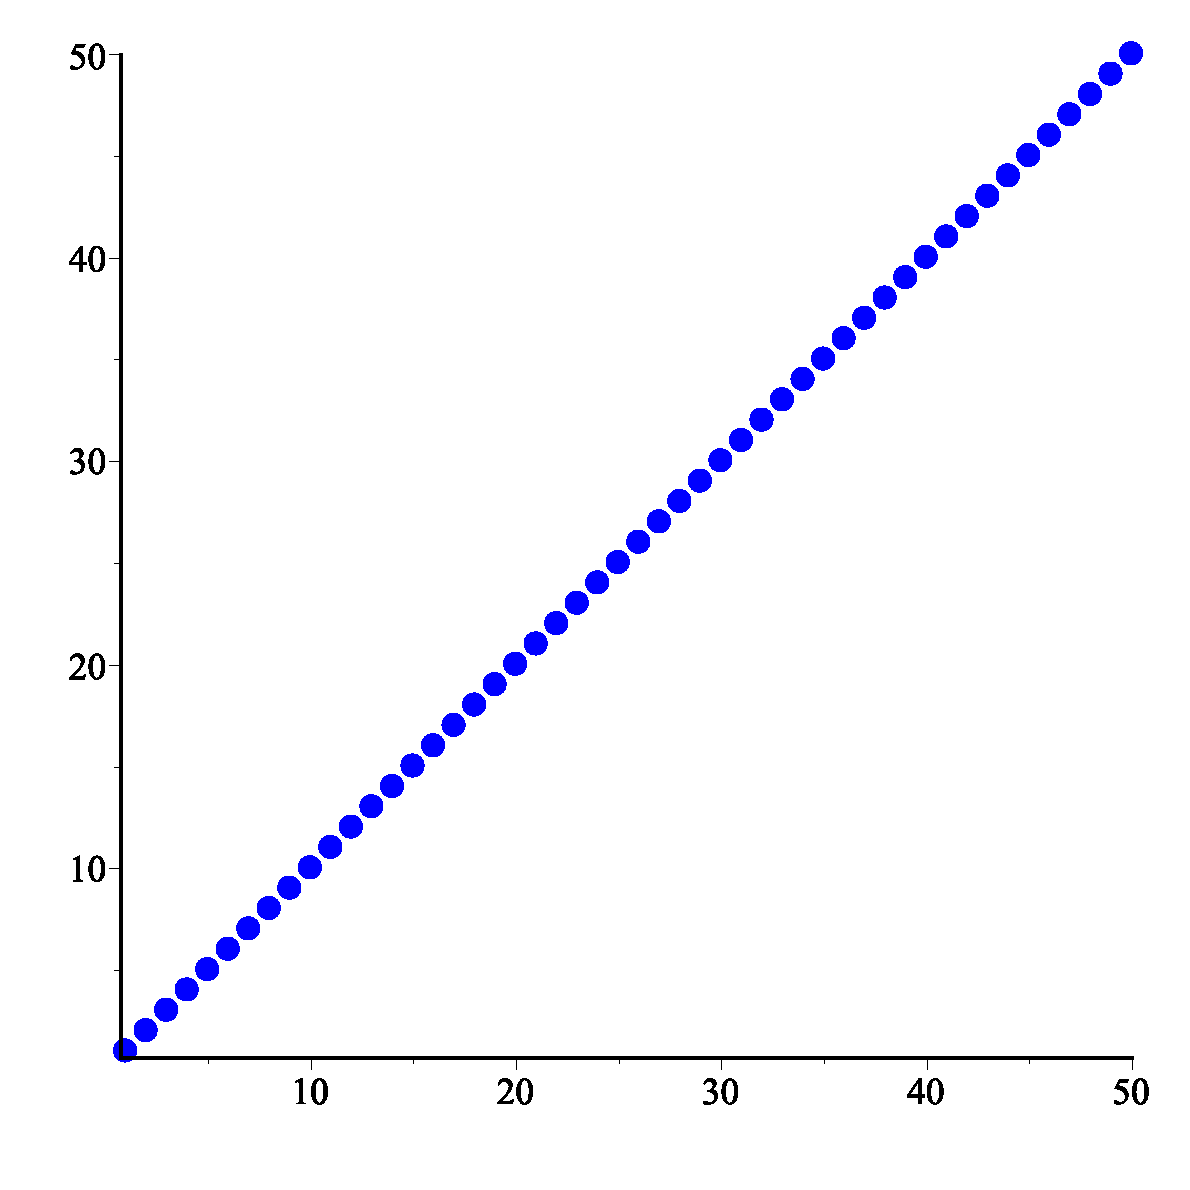
\includegraphics{figures/8_1_Sequence_n.eps}} 
%\end{center}
We recalling that a function $f$ has a limit $L$ at infinity if we can make the values of $f(x)$ as large as we want by choosing $x$ as large as we need. Since we can make the values of $n$ in our sequence as large as we want by choosing $n$ to be as large as we need, we suspect that this sequence does not have a limit as $n$ goes to infinity.

\item By observation we see that a formula for $s_n$ is $s_n = \frac{1}{n}$. A plot of the first 50 points in the sequence is shown here.
%\begin{center} \resizebox{!}{1.75in}{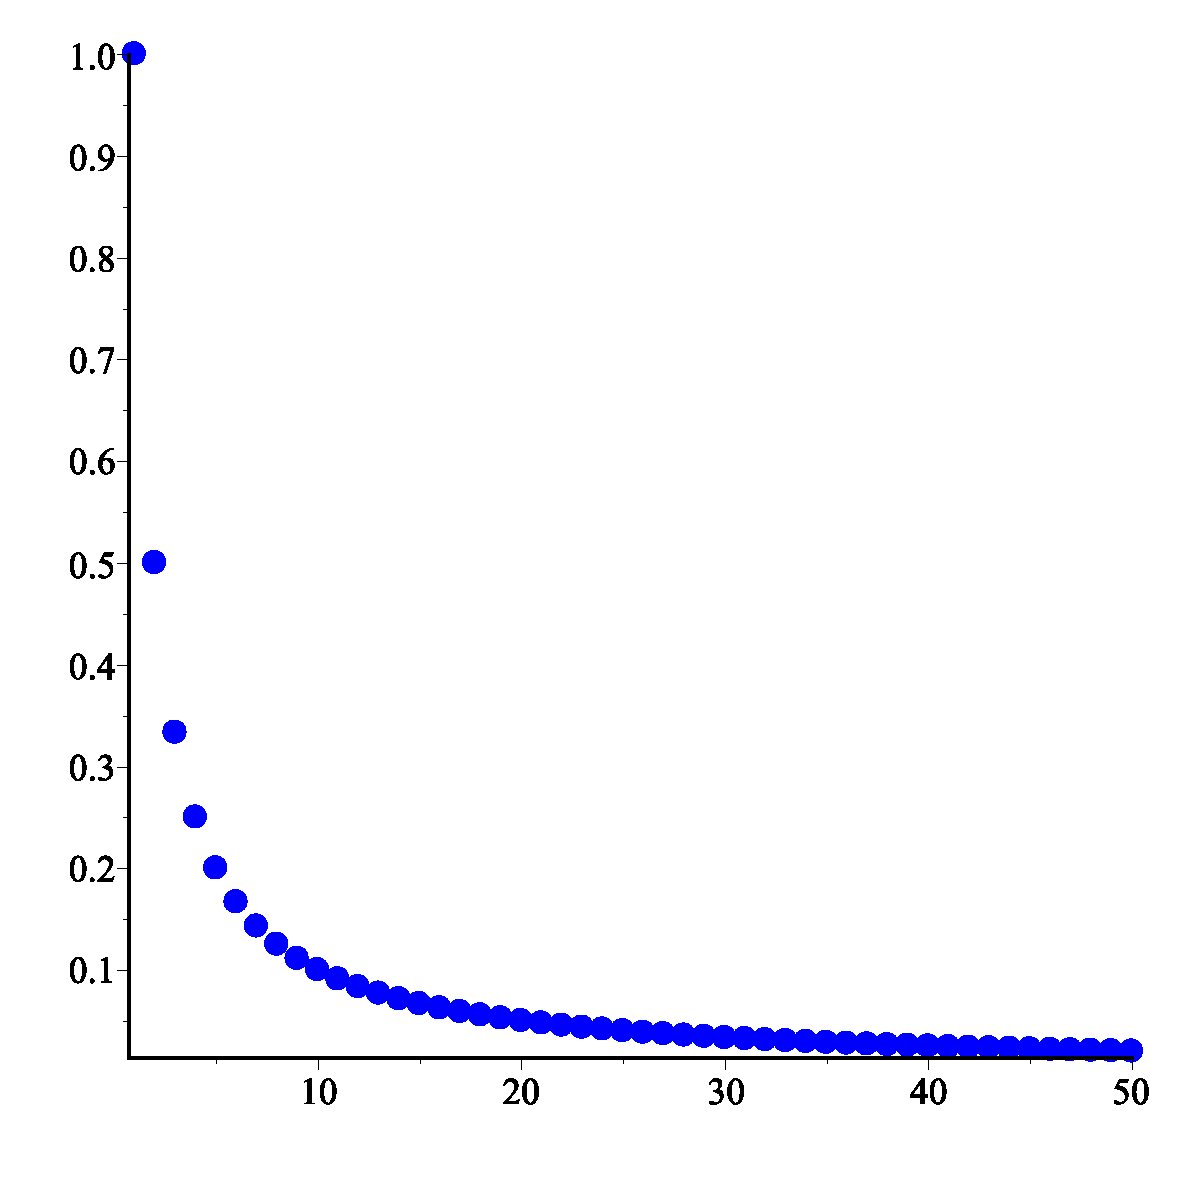
\includegraphics{figures/8_1_Sequence_1overn.eps}} \end{center}
Since we can make the values of $\frac{1}{n}$ in our sequence as close to 0 as we want by choosing $n$ to be as large as we need, we suspect that this sequence has a limit of 0 as $n$ goes to infinity.

\item Since the numerator is always 1 more than the denominator, a formula for $s_n$ is $s_n = \frac{n+1}{n}$. A plot of the first 50 points in the sequence is shown here.
%\begin{center} \resizebox{!}{1.75in}{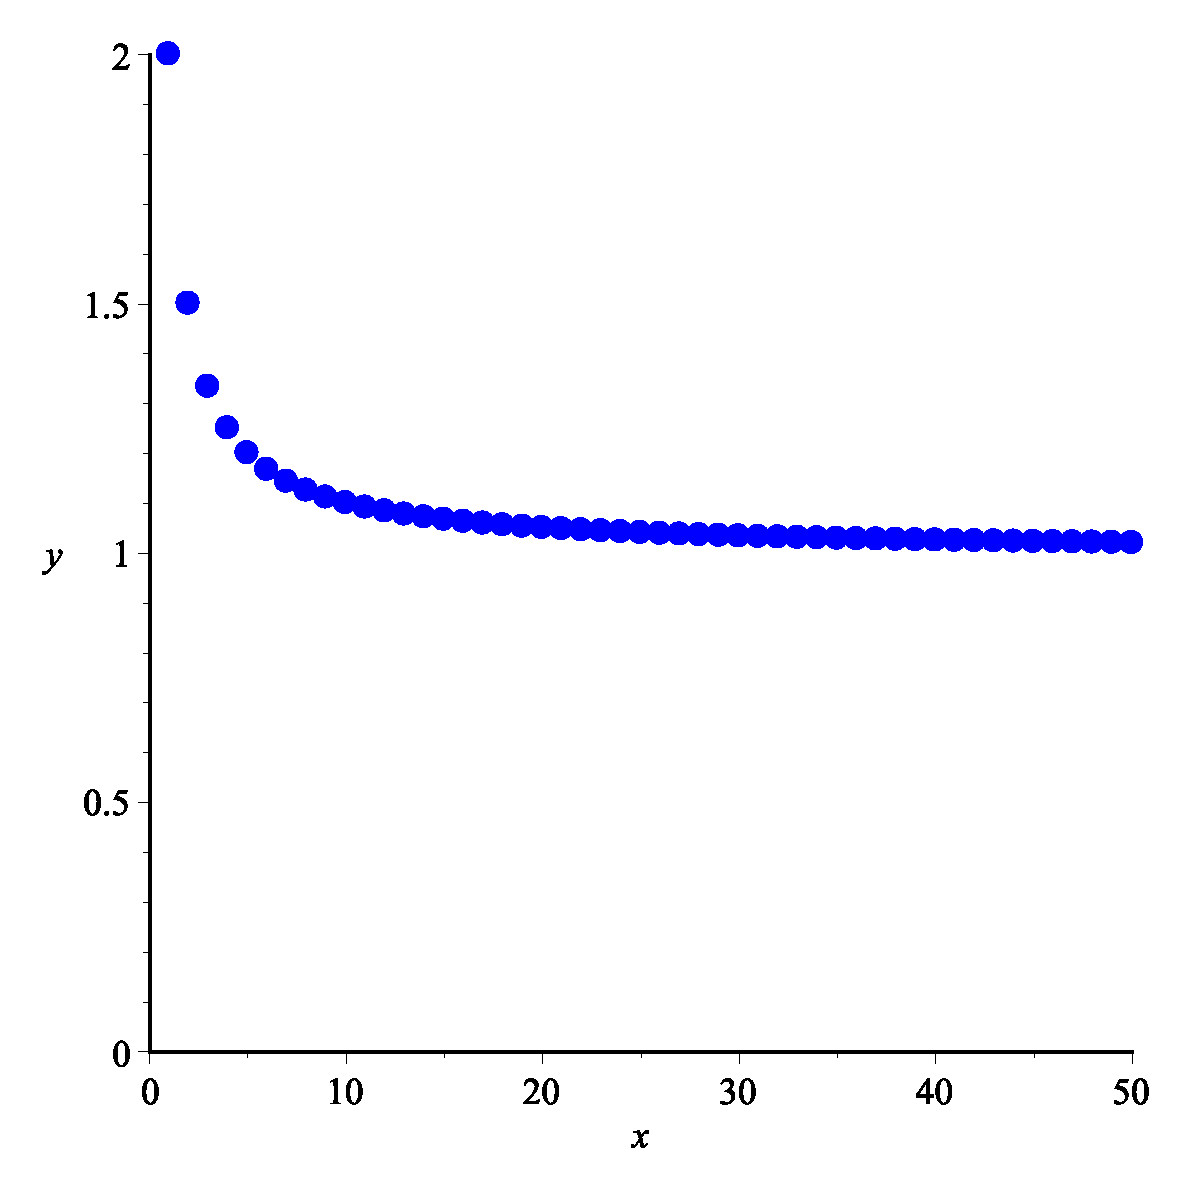
\includegraphics{figures/8_1_Sequence_nplus1overn.eps}} \end{center}
Since we can make the values of $\frac{n+1}{n}$ in our sequence as close to 1 as we want by choosing $n$ to be as large as we need, we suspect that this sequence has a limit of 1 as $n$ goes to infinity.

\ea
\end{activitySolution}
\aftera  % ACTIVITY

Next we formalize the ideas from Activity~\ref{7.1.Act1}.

\begin{activity} \label{7.1.Act2}
\ba
\item State clearly what it means for a continuous function $f$ to have a limit $L$ as $x \to \infty$.

\item Given that an infinite sequence of real numbers is a function from the integers to the real numbers, apply the idea from part (a) to explain what you think it means for a sequence $\{s_n\}$ to have a limit as $n \to \infty$.  

\item Based on your response to (b), decide if the sequence $\left\{ \frac{1+n}{2+n}\right\}$ has a limit as $n \to \infty$. If so, what is the limit? If not, why not?

\ea
\end{activity}

\begin{smallhint}
\ba
	\item Small hints for each of the prompts above.
\ea
\end{smallhint}
\begin{bighint}
\ba
	\item Big hints for each of the prompts above.
\ea
\end{bighint}
\begin{activitySolution}
\ba
	\item A continuous function $f$ has a limit $L$ as the independent variable $x$ goes to infinity if we can make the values of $f(x)$ as close to $L$ as we want by choosing $x$ as large as we need. 
    \item We expect that a sequence $\{s_n\}$ will have a limit $L$ as $n$ goes to infinity if we can make the entries $s_n$ in the sequence as close to $L$ as we want by choosing $n$ as large as we need.
    \item As $n$ gets large, the constant terms become infinitesimally small compared to $n$ and so $\frac{1+n}{2+n}$ looks like $\frac{n}{n}$ or 1 for large $n$. So the sequence $\left\{ \frac{1+n}{2+n}\right\}$ has a limit of 1 at infinity.   
\ea
\end{activitySolution}
\aftera  % ACTIVITY

In Activities \ref{7.1.Act1} and \ref{7.1.Act2} we investigated the notion of a sequence $\{s_n\}$ having a limit as $n$ goes to infinity. If a sequence $\{s_n\}$ has a limit as $n$ goes to infinity, we say that the sequence \emph{converges}\index{converge!sequence} or is a \emph{convergent sequence}\index{convergent sequence}. If the limit of a convergent sequence is the number $L$, we use the same notation as we did for continuous functions and write
\[\lim_{n \to \infty} s_n = L.\]
If a sequence $\{s_n\}$ does not converge then we say that the sequence $\{s_n\}$ \emph{diverges}\index{diverge!sequence}. Convergence of sequences is a major idea in this section and we describe it more formally as follows.

\concept{Convergence of a Sequence}{ % CONCEPT
A sequence $\{s_n\}$ of real numbers converges to a number $L$ if we can make all value of $s_k$ for $k \ge n$ as close to $L$ as we want by choosing $n$ to be sufficiently large.
} % end concept

Remember, the idea of sequence having a limit as $n \to \infty$ is the same as the idea of a continuous function having a limit as $x \to \infty$. The only new wrinkle here is that our sequences are discrete instead of continuous.

We conclude this section with a few more examples in the following activity.

\begin{activity} \label{7.1.Act3} Use graphical and/or algebraic methods to determine whether each of the following sequences converges or diverges.
\ba
\item $\ds \left\{\frac{1+2n}{3n-2}\right\}$


\item $\ds \left\{\frac{5+3^n}{10+2^n}\right\}$

\item $\ds \left\{\frac{10^n}{n!}\right\}$ (where $!$ is the \emph{factorial} symbol and $n! = n(n-1)(n-2) \cdots (2)(1)$ for any positive integer $n$ (as convention we define $0!$ to be 1)).

\ea
\end{activity}

\begin{smallhint}
\ba
	\item Small hints for each of the prompts above.
\ea
\end{smallhint}
\begin{bighint}
\ba
	\item Big hints for each of the prompts above.
\ea
\end{bighint}
\begin{activitySolution}
\ba
	\item A plot of the first 50 terms of the sequence $\left\{\frac{1+2n}{3n-2}\right\}$ is shown here.
\begin{center} \resizebox{!}{1.75in}{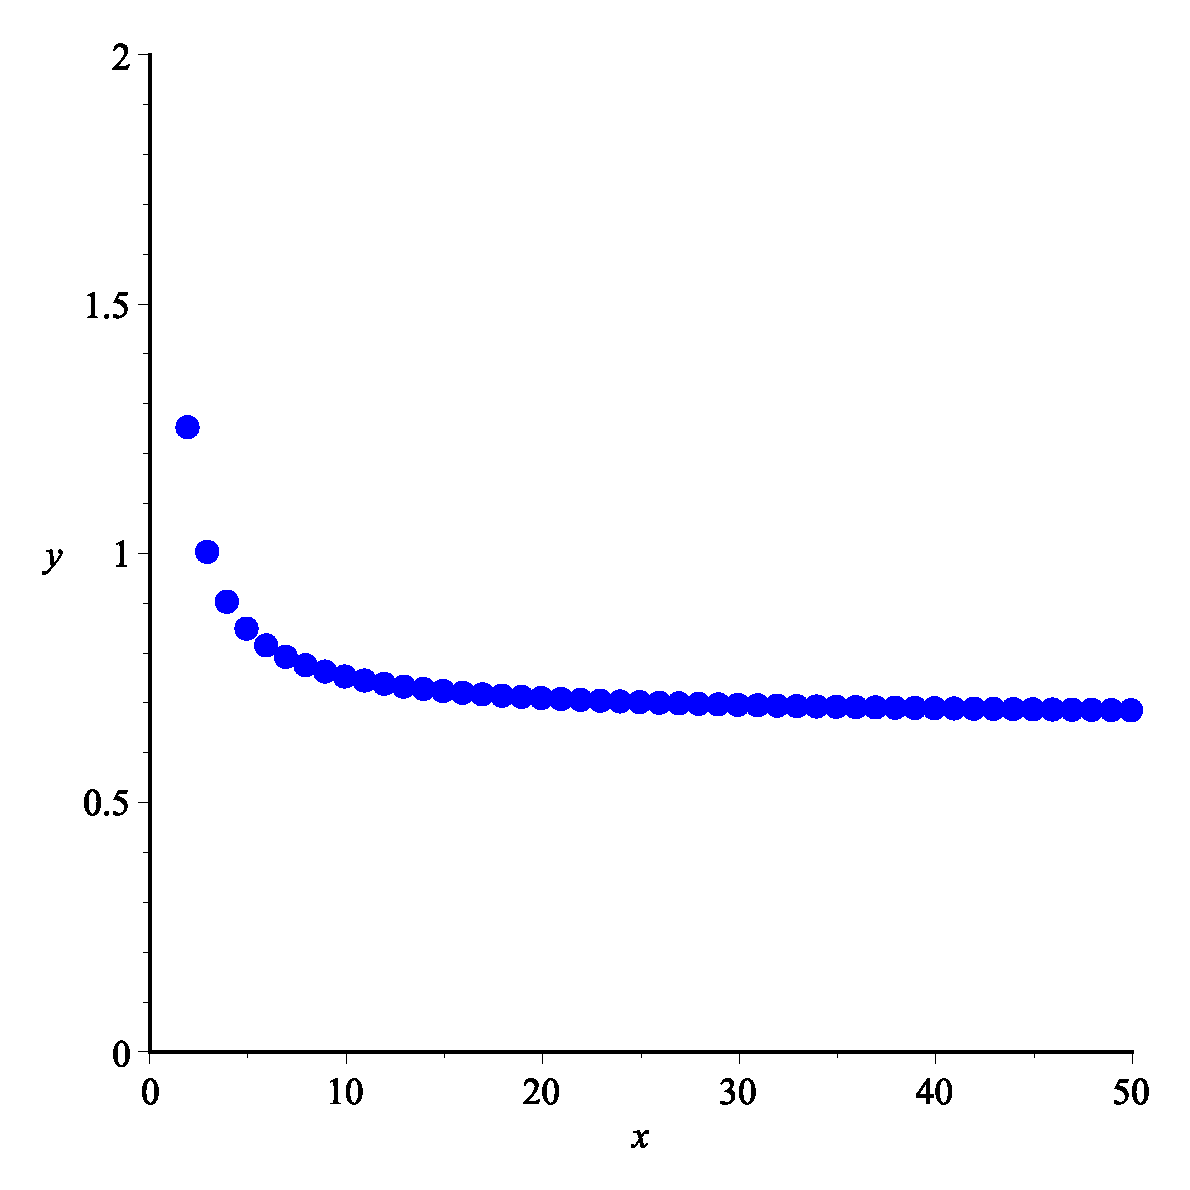
\includegraphics{figures/8_2_Sequence_a.eps}} \end{center}
The plot implies that the sequence has a limit between 0.5 and 1. For large $n$ the $2n$ term dominates the numerator and the $3n$ term the denominator. So $\frac{1+2n}{3n-2}$ looks like $\frac{2n}{3n} = \frac{2}{3}$ when $n$ is big. So the sequence $\left\{\frac{1+2n}{3n-2}\right\}$ converges to $\frac{2}{3}$.
    \item A plot of the first 50 terms of the sequence $\left\{\frac{5+3^n}{10+2^n}\right\}$ is shown here.
\begin{center} \resizebox{!}{1.75in}{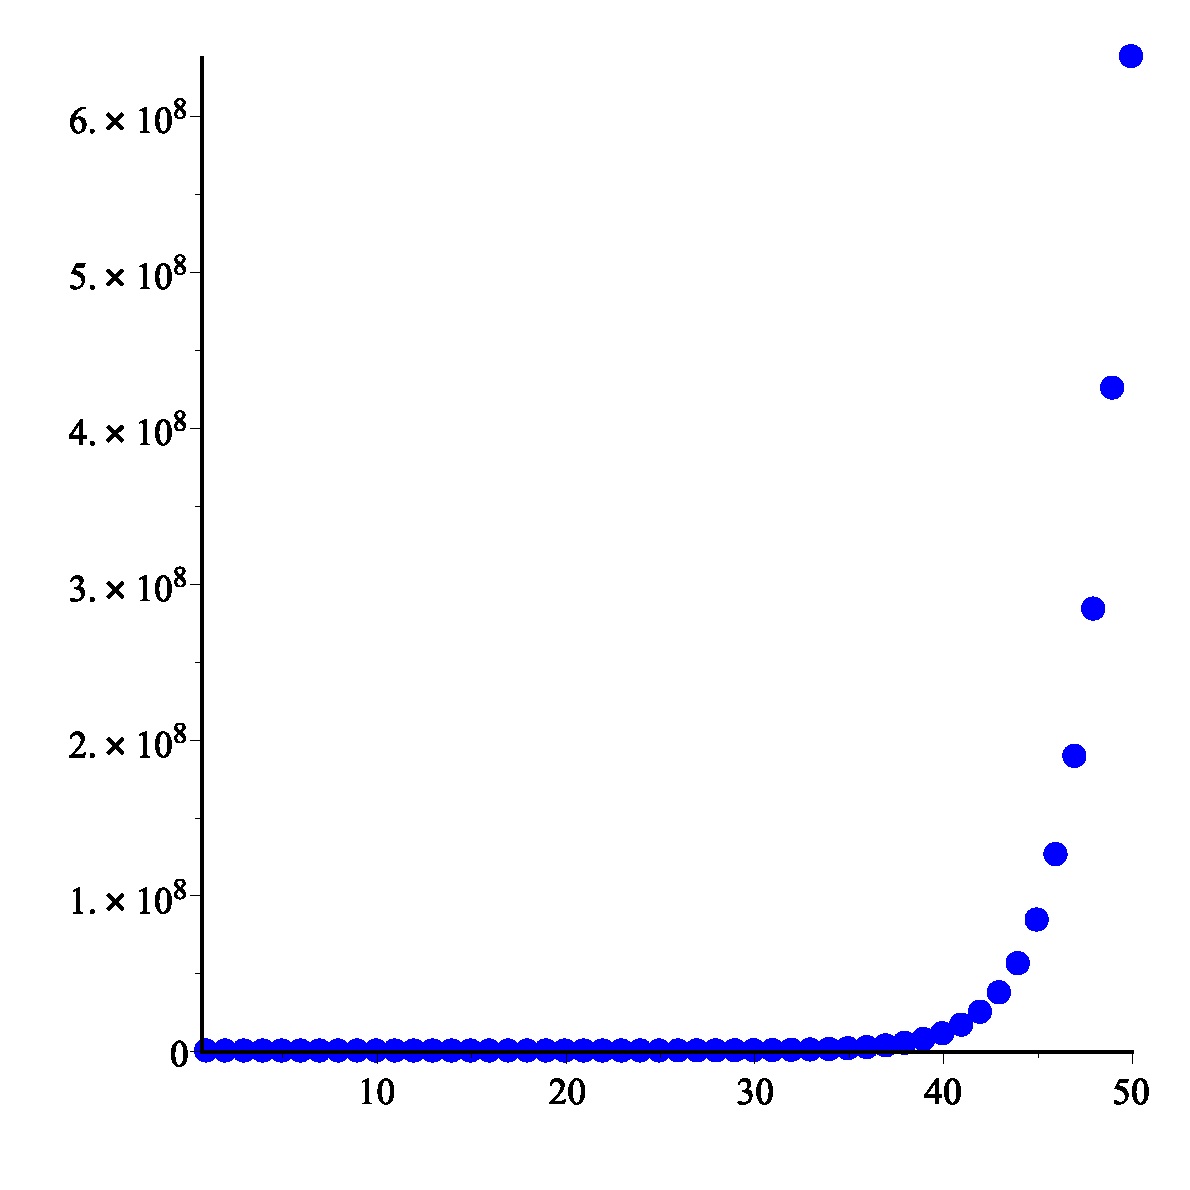
\includegraphics{figures/8_2_Sequence_b.eps}} \end{center}
The plot implies that the sequence does not have a limit as $n$ goes to infinity. For large $n$ the $3^n$ term dominates the numerator and the $2^n$ term the denominator. So $\frac{5+3^n}{10+2^n}$ looks like $\frac{3^n}{2^n} = \left(\frac{3}{2}\right)^n$ when $n$ is big. Since $\frac{3}{2} > 1$, the sequence $\left\{\frac{5+3^n}{10+2^n}\right\}$ diverges to infinity.
    \item A plot of the first 50 terms of the sequence $\left\{\frac{10^n}{n!}\right\}$ is shown here.
\begin{center} \resizebox{!}{1.75in}{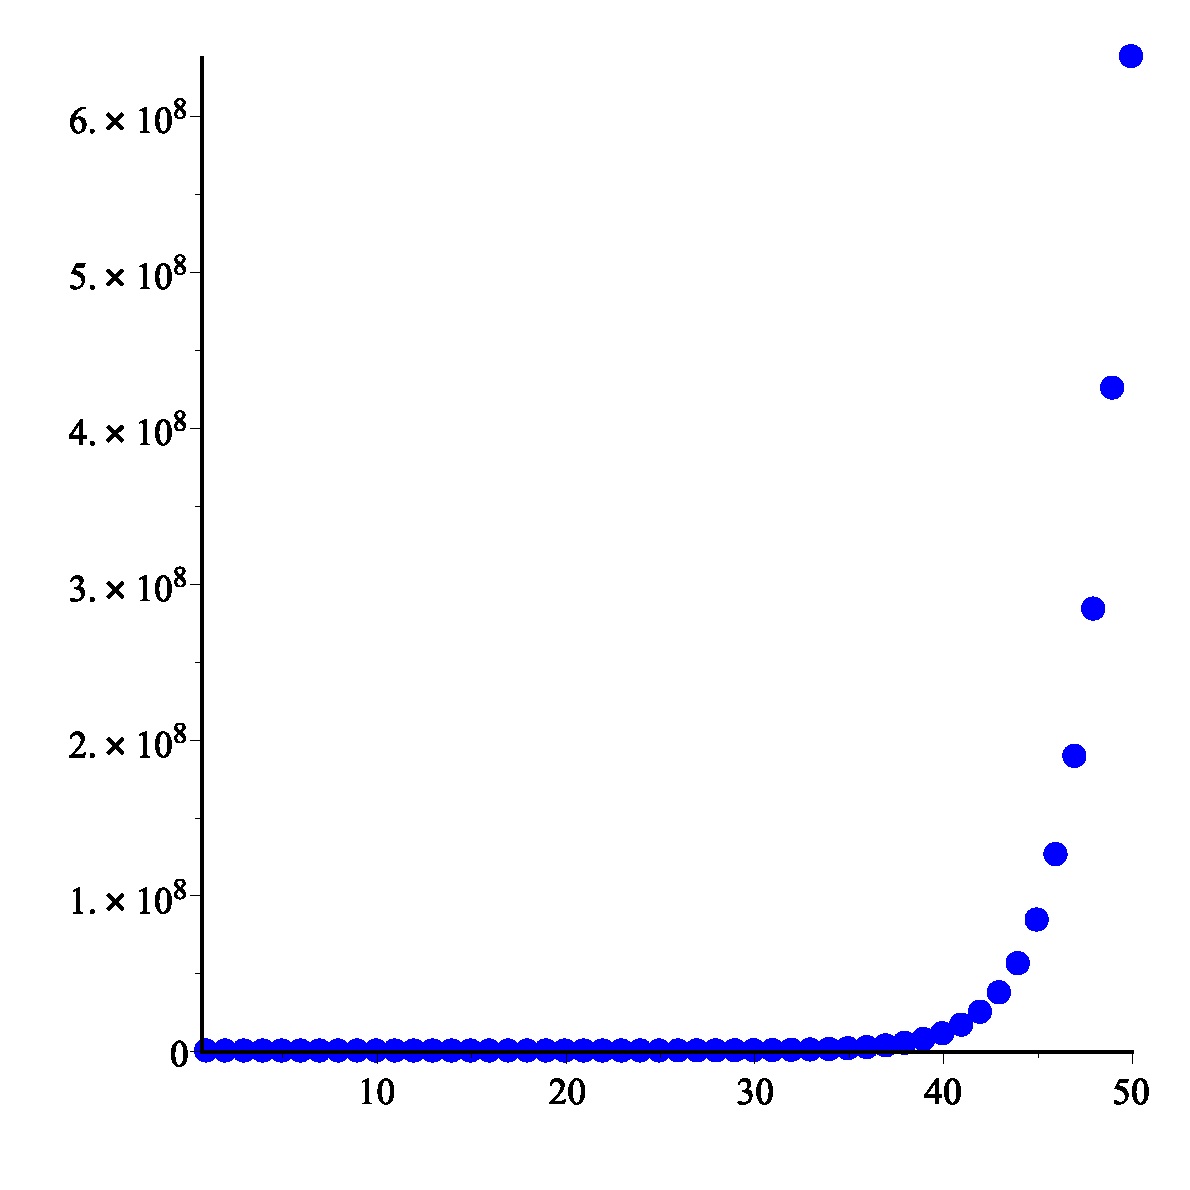
\includegraphics{figures/8_2_Sequence_b.eps}} \end{center}
Initially, it looks as though the terms increase without bound, but beginning at about $n=10$ the factorial in the denominator dominates the numerator. Notice that
 \[\frac{10^n}{n!} = \frac{10 \times 10 \times 10 \times \cdots \times 10}{1 \times 2 \times 3 \times \cdots n}\]
When $n > 20$, we have that $\frac{10}{n} < \frac{1}{2}$ and 
\begin{align*}
\frac{10^n}{n!} &= \left(\frac{10 \times 10 \times 10 \times \cdots \times 10}{1 \times 2 \times 3 \times \cdots 20}\right) \left(\frac{10 \times 10 \times 10 \times \cdots \times 10}{21 \times 22 \times 23 \times \cdots n}\right) \\
    &= \left(\frac{10^{20}}{20!}\right) \left(\frac{10}{21}\right) \left(\frac{10}{22}\right) \cdots \left(\frac{10}{n}\right)  \\
    &< \left(\frac{10^{20}}{20!}\right) \left(\frac{1}{2}\right)^{n-20}.
\end{align*}
Since $\frac{1}{2}<1$, the term $\left(\frac{1}{2}\right)^{n-20}$ goes to 0 as $n$ goes to infinity. The fact that $\frac{10^{20}}{20!}$ is a constant means that $\frac{10^n}{n!} \to 0$ as $n \to \infty$. 

\ea
\end{activitySolution}
\aftera  % ACTIVITY

%-------------
% SUMMARY
%-------------
\begin{summary}
\item A sequence is a list of objects in a specified order. We will typically work with sequences of real numbers and can also think of a sequence as a function from the positive integers to the set of real numbers.
\item A sequence $\{s_n\}$ of real numbers converges to a number $L$ if we can make every value of  $s_k$ for $k \ge n$ as close as we want to $L$ by choosing $n$ sufficiently large.
\item A sequence diverges if it does not converge.
\end{summary}